Special considerations are required for flow to convertible cells that can dry and rewet. When flow is between two cells that are wet, the head difference between them creates the driving force for flow. When the downstream cell is dry,
however, a reference elevation can be used instead of the downstream head to express flow between the nodes. The ``perched'' option in the Node Property Flow (NPF) Package can be used to correct downward flow to a partially saturated cell.

The ``flow correction'' option in the Multi-Aquifer Well (MAW) Package implements the same correction as the NPF package ``perched'' option and corrects the flow between a multi-aquifer well connection and a GWF cell. The approach used in the MAW Package is identical to the ``flow-to-dry-cell'' option available in \mfu~\citep{modflowusg}.

\subsection{Multi-Aquifer Well Flow Correction}

When the ``flow correction'' option is enabled, flow to a well from a GWF cell based on equation 7--50 in \cite{modflow6gwf} is

\begin{align}
	\label{eqn:mawQ}
	\mli{QMAW}_{\mli{MAW},n} = \begin{dcases}
		S_{\mli{MAW},n} C_{\mli{MAW},n}^0 \left( h_n - e_{\mli{MAW},n} \right) &  \mli{HMAW}_i < e_{\mli{MAW},n} \\
		S_{\mli{MAW},n} C_{\mli{MAW},n}^0 \left( h_n - \mli{HMAW}_{i} \right) & \mli{HMAW}_i \ge e_{\mli{MAW},n}
	\end{dcases} ,
\end{align}

\noindent where $S_{\mli{MAW},n}$ is the well screen saturation (unitless), $C_{\mli{MAW},n}^0$ is the saturated well conductance (\ulst), $h_n$ is the head in cell $n$ (\ul), $e_{\mli{MAW},n}$ is the reference elevation for the well connection (\ul), and $\mli{HMAW}_{i}$ is the head in well $i$ (\ul). The reference elevation for the well connection is defined to be

\begin{equation}
	\label{en}
	e_{\mli{MAW},n} = \begin{dcases}
		\mli{BOT}_n &  \mli{BOT}_n > \mli{BOT}_{\mli{MAW},n} \\
		\mli{BOT}_{\mli{MAW},n} &  \mli{BOT}_{\mli{MAW},n} > \mli{BOT}_n
	\end{dcases} ,
\end{equation}

\noindent where $\mli{BOT}_n$ is the bottom of cell $n$ (\ul) and $\mli{BOT}_{\mli{MAW},n}$ is the bottom of the well screen for the connection of well $i$ to cell $n$ (\ul). For the case where the head in cell $n$ is less than $e_{\mli{MAW},n}$, flow from a well to a GWF cell is

\begin{align}
	\label{eqn:mawQc2}
	\mli{QMAW}_{\mli{MAW},n} = \begin{dcases}
		S_{\mli{MAW},n} C_{\mli{MAW},n}^0 \left( e_{\mli{MAW},n} - \mli{HMAW}_{i}  \right) &  h_n < e_{\mli{MAW},n} \\
		S_{\mli{MAW},n} C_{\mli{MAW},n}^0 \left( h_n - \mli{HMAW}_{i} \right) & h_m \ge e_{\mli{MAW},n}
	\end{dcases} .
\end{align}

\subsection{Incorporation of the Flow Correction into the CVFD Groundwater Flow Equation}
Multi-aquifer well flow terms are incorporated into the CVFD flow equation \citep[eq. 6--1]{modflow6gwf} based on whether the standard or Newton-Raphson formulation is being used. The details of how the multi-aquifer well flow correction terms are incorporated into the CVFD flow equation is described below.

\subsubsection{Standard Formulation}

The terms in the standard flow equation for all groundwater cells connected to a multi-aquifer well $i$ based on \citep[eq. 7--55]{modflow6gwf} is

\begin{equation}
	\label{mawStdFlow}
	\sum\limits_{n \in \mli{MAW}_{i}}^{} S_{\mli{MAW},n} C_{\mli{MAW},n}^{0} \left( h_{n} - \mli{HMAW}_{i} \right) = 0 .
\end{equation}

\noindent To implement the flow correction, equation~\ref{eqn:mawQ} is modified to

\begin{align}
	\label{eqn:mawQfdc}
	\mli{QMAW}_{\mli{MAW},n} = S_{\mli{MAW},n} C_{\mli{MAW},n}^0 \left( h_n - \mli{HMAW}_{i} \right) + S_{\mli{MAW},n} C_{\mli{MAW},n}^0 \left( \mli{HMAW}_{i} - \overline{h}_{\mli{MAW},n} \right),
\end{align}

\noindent where $\overline{h}_{\mli{MAW},n}$ is a function that transitions between the head at the downstream node, $\mli{HMAW}_{i}$ in this case, and reference elevation $e_{\mli{MAW},n}$. The downstream head transition function used to correct the multi-aquifer flow for a connection is calculated as

\begin{align}
	\label{eqn:maw-hbar}
	\overline{h}_{\mli{MAW},n} = \begin{dcases}
		e_{\mli{MAW},n} &  h_{ds} < e_{\mli{MAW},n} \\
		h_{ds} & h_{ds} \ge e_{\mli{MAW},n}
	\end{dcases} ,
\end{align}

\noindent where $h_{ds}$ is head in the downstream node (\ul), which is the minimum of $\mli{HMAW}_{i}$ and $h_n$. The relation between the downstream head and $\overline{h}_{\mli{MAW},n}$ is shown in figure~\ref{fig:mawhbar}.

\begin{figure}[!ht]
	\begin{center}
	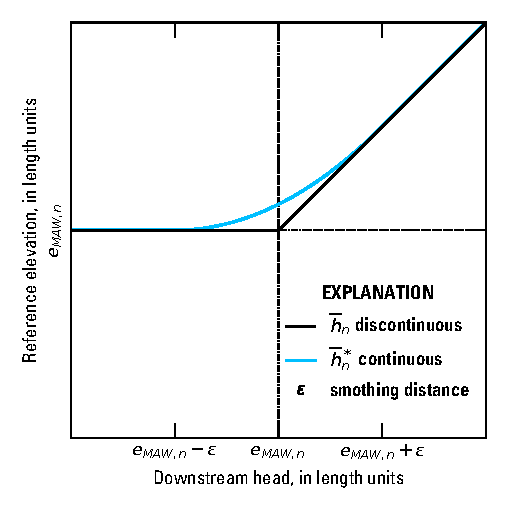
\includegraphics{./Figures/MAWDischargeCorrection.pdf}
	\caption[Graph showing the downstream head transition functions used to correct the multi-aquifer flow for a connection]{Graph showing the discontinuous (eq.~\ref{eqn:maw-hbar}) and continuous (eq.~\ref{eqn:maw-chbar})  downstream head transition function used to correct the multi-aquifer flow for a connection as it transitions from saturated to partially saturated conditions. The interval over which the smoothing occurs, $\epsilon$, is also shown}
	\label{fig:mawhbar}
	\end{center}
\end{figure}

Similarly, when $h_n$ is the downstream node equation~\ref{eqn:mawQc2} is modified to

\begin{align}
	\label{eqn:mawQfdc2}
	\mli{QMAW}_{\mli{MAW},n} = S_{\mli{MAW},n} C_{\mli{MAW},n}^0 \left( h_n - \mli{HMAW}_{i} \right) + S_{\mli{MAW},n} C_{\mli{MAW},n}^0 \left( \overline{h}_{\mli{MAW},n} - h_n \right),
\end{align}

The first term on the right hand side of equations~\ref{eqn:mawQfdc} and~\ref{eqn:mawQfdc2} ($S_{\mli{MAW},n} C_{\mli{MAW},n}^0$) are added to the coefficient matrix used to solve the coupled groundwater and multi-aquifer well flow equations as part of the standard MAW package formulation \citep[eq. 7--55]{modflow6gwf}. The flow correction is made by subtracting the second term on the right hand side of equations~\ref{eqn:mawQfdc} and~\ref{eqn:mawQfdc2} from the right had side of equation 6--1 in \cite{modflow6gwf}. In the case where $\mli{HMAW}_{i}$ and $h_n$ are both greater than $e_{\mli{MAW},n}$, the second term on the right hand side of equations~\ref{eqn:mawQfdc} and~\ref{eqn:mawQfdc2} is equal to zero, which results in a equation identical to equation~\ref{mawStdFlow} for a single connection.


\subsubsection{Newton-Raphson Formulation}

The modified Newton-Raphson form of equation~\ref{mawStdFlow} solved for a single connection in terms of $h$ instead of $\Delta h$  and incorporated into the Newton-Raphson form of the groundwater flow equation \citep[eq. 2--26]{modflow6gwf} is

\begin{equation}
	\label{eqn:nrMawQ}
	\begin{aligned}
		\frac{\partial \mli{QMAW}_{\mli{MAW},n}}{\partial \mli{HMAW}_i}  \mli{HMAW}_i^k + &\frac{\partial \mli{QMAW}_{\mli{MAW},n}}{\partial h_n}  h^k_n = - \mli{QMAW}_{\mli{MAW},n} + \\
		&\frac{\partial \mli{QMAW}_{\mli{MAW},n}}{\partial \mli{HMAW}_i}  \mli{HMAW}_i^{k-1} +  \frac{\partial \mli{QMAW}_{\mli{MAW},n}}{\partial h_n}  h^{k-1}_n ,
	\end{aligned}
\end{equation}

\noindent where $\mli{HMAW}_i^k$ and $h^k_n$ are the heads at the end of the current non-linear (picard) iteration and $\mli{HMAW}_i^{k-1}$ and $h^{k-1}_n$ are the head at the start of the current non-linear iteration.

When the Newton-Raphson formulation is used, discontinuous derivatives can cause non-convergence in the neighborhood of the discontinuity \citep{doi:10.1029/2006WR005195}. As a result, the discontinuous well screen saturation ($S_{\mli{MAW},n}$) in equations~\ref{eqn:mawQfdc} and~\ref{eqn:mawQfdc2} is replaced by a quadratically smoothed well screen saturation ($S_{\mli{MAW},n}^*$ -- eq. 4--5 in \cite{modflow6gwf}). The discontinuous downstream head transition function ($\overline{h}_{\mli{MAW},n}$, eq.~\ref{eqn:maw-hbar}) in equations~\ref{eqn:mawQfdc} and~\ref{eqn:mawQfdc2} is also replaced by

\begin{align}
	\label{eqn:maw-chbar}
	\overline{h}_{\mli{MAW},n}^* = \begin{dcases}
		e_{\mli{MAW},n} &  h_{ds} - e_{\mli{MAW},n} < -\epsilon \\
		\frac{( h_{ds} - e_{\mli{MAW},n} )^2}{4 \epsilon} + \frac{( h_{ds} - e_{\mli{MAW},n} )}{2} + \frac{\epsilon}{4} + e_{\mli{MAW},n}  & -\epsilon < h_{ds} - e_{\mli{MAW},n} < +\epsilon \\
		h_{ds} & h_{ds} - e_{\mli{MAW},n} \ge +\epsilon
	\end{dcases} ,
\end{align}

\noindent where $\epsilon$ is the interval over which the head transition function is smoothed. The relation between the downstream head and $\overline{h}^*_{\mli{MAW},n}$ is shown in figure~\ref{fig:mawhbar}. Simplification of equations~\ref{eqn:mawQfdc} and~\ref{eqn:mawQfdc2} results in

\begin{align}
	\label{eqn:mawQNRc}
	\mli{QMAW}_{\mli{MAW},n} = S_{\mli{MAW},n}^* C_{\mli{MAW},n}^0 \left( h_n - \overline{h}^*_{\mli{MAW},n} \right)
\end{align}

\noindent and

\begin{align}
	\label{eqn:mawQNRc2}
	\mli{QMAW}_{\mli{MAW},n} = S_{\mli{MAW},n}^* C_{\mli{MAW},n}^0 \left( \overline{h}^*_{\mli{MAW},n} - \mli{HMAW}_{i} \right)
\end{align}

\noindent when $\mli{HMAW}_i$ and $h_n$ are the downstream heads, respectively. The derivatives of equation~\ref{eqn:mawQNRc} with respect to $h_n$ and $\mli{HMAW}_i$ are

\begin{equation}
	\label{eqn:nrMawdQdh1}
	\frac{\partial \mli{QMAW}_{\mli{MAW},n}}{\partial \mli{HMAW}_i} =  -S_{\mli{MAW},n}^* C_{\mli{MAW},n}^0 \frac{\partial \overline{h}^*_{\mli{MAW},n}}{{\partial \mli{HMAW}_i}}
\end{equation}

\noindent and

\begin{equation}
	\label{eqn:nrMawdQdhmaw1}
	\frac{\partial \mli{QMAW}_{\mli{MAW},n}}{\partial h_n} = S_{\mli{MAW},n}^* C_{\mli{MAW},n}^0 + \frac{\partial S_{\mli{MAW},n}^*}{\partial h_n} C_{\mli{MAW},n}^0 \left( h_n - \overline{h}^*_{\mli{MAW},n} \right) ,
\end{equation}

\noindent respectively. The derivatives of equation~\ref{eqn:mawQNRc2} with respect to $h_n$ and $\mli{HMAW}_i$ are

\begin{equation}
	\label{eqn:nrMawdQdh2}
	\frac{\partial \mli{QMAW}_{\mli{MAW},n}}{\partial \mli{HMAW}_i} =  -S_{\mli{MAW},n}^* C_{\mli{MAW},n}^0 + \frac{\partial S_{\mli{MAW},n}^*}{\partial \mli{HMAW}_i} C_{\mli{MAW},n}^0 \left( \overline{h}^*_{\mli{MAW},n} - \mli{HMAW}_{i} \right)
	\end{equation}

\noindent and

\begin{equation}
	\label{eqn:nrMawdQdhmaw2}
	\frac{\partial \mli{QMAW}_{\mli{MAW},n}}{\partial h_n} =  S_{\mli{MAW},n}^* C_{\mli{MAW},n}^0 \frac{\partial \overline{h}^*_{\mli{MAW},n}}{\partial h_n} .
\end{equation}

The derivative of $\overline{h}^*_{\mli{MAW},n}$ with respect to the downstream head is

\begin{align}
	\label{eqn:maw-cdhbar}
	\frac{\partial \overline{h}^*_{\mli{MAW},n}}{\partial h_{ds}} = \begin{dcases}
		0 &  h_{ds} - e_{\mli{MAW},n} < -\epsilon \\
		\frac{h_{ds} - e_{\mli{MAW},n}}{2 \epsilon} + \frac{1}{2} & -\epsilon < h_{ds} - e_{\mli{MAW},n} < +\epsilon \\
		1 & h_{ds} - e_{\mli{MAW},n} \ge +\epsilon
	\end{dcases} .
\end{align}


\paragraph{Newton-Raphson formulation when $\mli{HMAW}_i$ is the Downstream Head}

The Newton-Raphson form of the equation~\ref{eqn:mawQfdc}, when $\mli{HMAW}_i$ is the downstream head, is formulated by substituting equations~\ref{eqn:mawQNRc}, ~\ref{eqn:nrMawdQdh1}, and ~\ref{eqn:nrMawdQdhmaw1} into equation~\ref{eqn:nrMawQ}, which results in

\begin{equation}
	\label{eqn:nrMawQmawds01}
	\begin{aligned}
		\biggl[ -S_{\mli{MAW},n}^* &C_{\mli{MAW},n}^0 \frac{\partial \overline{h}^*_{\mli{MAW},n}}{{\partial \mli{HMAW}_i}}
 \biggr] \mli{HMAW}_i^k + \\
 		&\biggl[ S_{\mli{MAW},n}^* C_{\mli{MAW},n}^0 + \frac{\partial S_{\mli{MAW},n}^*}{\partial h_n} C_{\mli{MAW},n}^0 \left( h_n^{k-1} - \overline{h}_{\mli{MAW},n}^{*k-1} \right) \biggr]  h^k_n = \\
		&-S_{\mli{MAW},n}^* C_{\mli{MAW},n}^0 \left( h_n^{k-1} - \overline{h}_{\mli{MAW},n}^{*k-1} \right) + \\
		&\biggl[ -S_{\mli{MAW},n}^* C_{\mli{MAW},n}^0 \frac{\partial \overline{h}^*_{\mli{MAW},n}}{{\partial \mli{HMAW}_i}}
 \biggr] \mli{HMAW}_i^{k-1} + \\
 		&\biggl[ S_{\mli{MAW},n}^* C_{\mli{MAW},n}^0 + \frac{\partial S_{\mli{MAW},n}^*}{\partial h_n} C_{\mli{MAW},n}^0 \left( h_n^{k-1} - \overline{h}_{\mli{MAW},n}^{*k-1} \right) \biggr]  h^{k-1}_n .
	\end{aligned}
\end{equation}

\noindent Simplifying equation~\ref{eqn:nrMawQmawds01} results in

\begin{equation}
	\label{eqn:nrMawQmawds02}
	\begin{aligned}
		\biggl[ -S_{\mli{MAW},n}^* &C_{\mli{MAW},n}^0 \frac{\partial \overline{h}^*_{\mli{MAW},n}}{{\partial \mli{HMAW}_i}}
 \biggr] \mli{HMAW}_i^k + \\
 		&\biggl[ S_{\mli{MAW},n}^* C_{\mli{MAW},n}^0 + \frac{\partial S_{\mli{MAW},n}^*}{\partial h_n} C_{\mli{MAW},n}^0 \left( h_n^{k-1} - \overline{h}_{\mli{MAW},n}^{*k-1} \right) \biggr]  h^k_n = \\
		&S_{\mli{MAW},n}^* C_{\mli{MAW},n}^0 \overline{h}_{\mli{MAW},n}^{*k-1} + \biggl[ -S_{\mli{MAW},n}^* C_{\mli{MAW},n}^0 \frac{\partial \overline{h}^*_{\mli{MAW},n}}{{\partial \mli{HMAW}_i}}
 \biggr] \mli{HMAW}_i^{k-1} + \\
 		&\biggl[ \frac{\partial S_{\mli{MAW},n}^*}{\partial h_n} C_{\mli{MAW},n}^0 \left( h_n^{k-1} - \overline{h}_{\mli{MAW},n}^{*k-1} \right) \biggr]  h^{k-1}_n .
	\end{aligned}
\end{equation}

\noindent To complete the Newton-Raphson formulation the terms added to the coefficient matrix and right-hand side during the standard formulation step (eq.~\ref{eqn:mawQfdc}) are modified by adding

\begin{equation}
	\label{eqn:nrMawdsdiag}
	S_{\mli{MAW},n}^* C_{\mli{MAW},n}^0 \left( 1 - \frac{\partial \overline{h}^*_{\mli{MAW},n}}{{\partial \mli{HMAW}_i}} \right)
\end{equation}

\noindent to the diagonal position in the row for multi-aquifer well $i$, adding

\begin{equation}
	\label{eqn:nrMawdsoffd}
	\frac{\partial S_{\mli{MAW},n}^*}{\partial h_n} C_{\mli{MAW},n}^0 \left( h_n - \overline{h}^*_{\mli{MAW},n} \right)
\end{equation}

\noindent to the off-diagonal position for GWF cell $n$ in the row for multi-aquifer well $i$, and adding

\begin{equation}
	\label{eqn:nrMawdsrhs}
	S_{\mli{MAW},n}^* C_{\mli{MAW},n}^0 \left( 1 - \frac{\partial \overline{h}^*_{\mli{MAW},n}}{{\partial \mli{HMAW}_i}} \right) \mli{HMAW}_i^{k-1} + \frac{\partial S_{\mli{MAW},n}^*}{\partial h_n} C_{\mli{MAW},n}^0 \left( h_n - \overline{h}^*_{\mli{MAW},n} \right) h_n^{k-1}
\end{equation}

\noindent to the right-hand side in the row for multi-aquifer well $i$. The $\left( 1 - \frac{\partial \overline{h}^*_{\mli{MAW},n}}{{\partial \mli{HMAW}_i}} \right)$ term in equation~\ref{eqn:nrMawdsdiag} removes the $-S_{\mli{MAW},n}^* C_{\mli{MAW},n}^0$ term added during standard formulation step and correctly adds the $-S_{\mli{MAW},n}^* C_{\mli{MAW},n}^0 \frac{\partial \overline{h}^*_{\mli{MAW},n}}{{\partial \mli{HMAW}_i}}$ term. The row for the connected groundwater cell (row $n$) is also modified by subtracting equations~\ref{eqn:nrMawdsdiag}, ~\ref{eqn:nrMawdsoffd}, and~\ref{eqn:nrMawdsrhs} from the off-diagonal (column corresponding to multi-aquifer well $i$), diagonal, and right-hand side, respectively.

\paragraph{Newton-Raphson formulation when $h_n$ is the Downstream Head}

The Newton-Raphson form of the equation~\ref{eqn:mawQfdc2}, when $h_n$ is the downstream head, is formulated by substituting equations ~\ref{eqn:mawQNRc2}, ~\ref{eqn:nrMawdQdh2}, and ~\ref{eqn:nrMawdQdhmaw2} into equation~\ref{eqn:nrMawQ}, which results in

\begin{equation}
	\label{eqn:nrMawQgwfds01}
	\begin{aligned}
		\biggl[ -S_{\mli{MAW},n}^* &C_{\mli{MAW},n}^0 + \frac{\partial S_{\mli{MAW},n}^*}{\partial \mli{HMAW}_i} C_{\mli{MAW},n}^0 \left( \overline{h}_{\mli{MAW},n}^{*k-1} - \mli{HMAW}_{i}^{k-1} \right)  \biggr] \mli{HMAW}_i^k + \\
		&\biggl[ S_{\mli{MAW},n}^* C_{\mli{MAW},n}^0 \frac{\partial \overline{h}^*_{\mli{MAW},n}}{\partial h_n} \biggr]  h^k_n = - S_{\mli{MAW},n}^* C_{\mli{MAW},n}^0 \left( \overline{h}_{\mli{MAW},n}^{*k-1} - \mli{HMAW}_{i}^{k-1} \right) + \\
		&\biggl[ -S_{\mli{MAW},n}^* C_{\mli{MAW},n}^0 + \frac{\partial S_{\mli{MAW},n}^*}{\partial \mli{HMAW}_i} C_{\mli{MAW},n}^0 \left( \overline{h}_{\mli{MAW},n}^{*k-1} - \mli{HMAW}_{i}^{k-1} \right) \biggr] \mli{HMAW}_i^{k-1} + \\ &
		\biggl[ S_{\mli{MAW},n}^* C_{\mli{MAW},n}^0 \frac{\partial \overline{h}^*_{\mli{MAW},n}}{\partial h_n} \biggr]  h^{k-1}_n .
	\end{aligned}
\end{equation}

\noindent Simplifying equation~\ref{eqn:nrMawQgwfds01} results in

\begin{equation}
	\label{eqn:nrMawQgwfds02}
	\begin{aligned}
		\biggl[ -S_{\mli{MAW},n}^* &C_{\mli{MAW},n}^0 + \frac{\partial S_{\mli{MAW},n}^*}{\partial \mli{HMAW}_i} C_{\mli{MAW},n}^0 \left( \overline{h}_{\mli{MAW},n}^{*k-1} - \mli{HMAW}_{i}^{k-1} \right)  \biggr] \mli{HMAW}_i^k + \\
		&\biggl[ S_{\mli{MAW},n}^* C_{\mli{MAW},n}^0 \frac{\partial \overline{h}^*_{\mli{MAW},n}}{\partial h_n} \biggr]  h^k_n = - S_{\mli{MAW},n}^* C_{\mli{MAW},n}^0 \overline{h}_{\mli{MAW},n}^{*k-1} + \\
		&\biggl[ \frac{\partial S_{\mli{MAW},n}^*}{\partial \mli{HMAW}_i} C_{\mli{MAW},n}^0 \left( \overline{h}_{\mli{MAW},n}^{*k-1} - \mli{HMAW}_{i}^{k-1} \right) \biggr] \mli{HMAW}_i^{k-1} + \\ &
		\biggl[ S_{\mli{MAW},n}^* C_{\mli{MAW},n}^0 \frac{\partial \overline{h}^*_{\mli{MAW},n}}{\partial h_n} \biggr]  h^{k-1}_n .
	\end{aligned}
\end{equation}

\noindent To complete the Newton-Raphson formulation the terms added to the coefficient matrix and right-hand side during the standard formulation step (eq.~\ref{eqn:mawQfdc2}) are modified by adding

\begin{equation}
	\label{eqn:nrGwfdsdiag}
	\frac{\partial S_{\mli{MAW},n}^*}{\partial \mli{HMAW}_i} C_{\mli{MAW},n}^0 \left( \overline{h}_{\mli{MAW},n}^{*k-1} - \mli{HMAW}_{i}^{k-1} \right)
\end{equation}

\noindent to the diagonal position in the row for multi-aquifer well $i$, adding

\begin{equation}
	\label{eqn:nrGwfdsoffd}
	S_{\mli{MAW},n}^* C_{\mli{MAW},n}^0 \left( \frac{\partial \overline{h}^*_{\mli{MAW},n}}{\partial h_n} - 1\right)
\end{equation}

\noindent to the off-diagonal position for GWF cell $n$ in the row for multi-aquifer well $i$, and adding

\begin{equation}
	\label{eqn:nrGwfdsrhs}
	\frac{\partial S_{\mli{MAW},n}^*}{\partial \mli{HMAW}_i} C_{\mli{MAW},n}^0 \left( \overline{h}_{\mli{MAW},n}^{*k-1} - \mli{HMAW}_{i}^{k-1} \right) \mli{HMAW}_i^{k-1} + S_{\mli{MAW},n}^* C_{\mli{MAW},n}^0 \left( \frac{\partial \overline{h}^*_{\mli{MAW},n}}{\partial h_n} - 1 \right) h^{k-1}_n
\end{equation}

\noindent to the right-hand side in the row for multi-aquifer well $i$. The $\left( \frac{\partial \overline{h}^*_{\mli{MAW},n}}{\partial h_n} - 1 \right)$ term in equation~\ref{eqn:nrGwfdsoffd} removes the $S_{\mli{MAW},n}^* C_{\mli{MAW},n}^0$ term added during standard formulation step and correctly adds the $S_{\mli{MAW},n}^* C_{\mli{MAW},n}^0 \frac{\partial \overline{h}^*_{\mli{MAW},n}}{{\partial h_n}}$ term. The row for the connected groundwater cell (row $n$) is also modified by subtracting equations~\ref{eqn:nrGwfdsdiag}, ~\ref{eqn:nrGwfdsoffd}, and~\ref{eqn:nrGwfdsrhs} from the off-diagonal (column corresponding to multi-aquifer well $i$), diagonal, and right-hand side, respectively.